% ARGUES: the judge was validated, it drifted, the drift was caught, its
%         differentiality was tested rather than assumed, and a paired sub-study
%         measured the misclassification directly.
% DRAWS FROM: docs/judge_drift_disclosure_draft.md (fully refreshed 2026-08-30),
%             docs/drift_interaction_prespec.md (locked before any model was fit),
%             data/analysis/phase_c/drift_interaction.json,
%             data/analysis/phase_c/rejudge_substudy_result.json,
%             the judge-validation artifacts.
% STATUS: every figure below was re-run at the complete 31,980 judgments on
%         2026-08-30 and is final. Nothing here is gated on further collection.
%
% This section is a contribution, not a confession. Concurrent work reports no
% drift analysis at all. Write it as methodology for LLM-judge pipelines.

\section{Instrument validity}
\label{sec:instrument}

\subsection{Judge validation}

The outcome variable is produced by an LLM judge, so the judge is part of what
has to be validated. Two hand-checks were run, and they answer different
questions.

The pre-registered gate required at least 90\% three-way agreement with blind
hand-checked labels before the judge could be used at scale. On a 50-citation
blind check it reached \textbf{96.0\%} $[86.5, 98.9]$, clearing the gate. The
comparison that makes that number meaningful is not the gate but the alternative:
the \textbf{structured verifier alone scores 46.0\%} $[33.0, 59.6]$ on the same
citations. The judge layer takes the pipeline from 46\% to 96\%, and that
contribution is unambiguous.

What the 96\% could not do is distinguish the pipeline from a judge that says
REAL to everything. That check set was 88\% REAL with only six fabrication
events, so a trivial always-REAL baseline scores 88\% against the pipeline's
96\%: a four-citation margin, exact McNemar $p = 0.125$. Passing a gate against
labels is not the same as beating the degenerate strategy.

So a second, fabrication-enriched validation was run on the Phase C corpus
itself: 150 citations drawn across four strata with design weights, labeled
blind, with no pipeline evidence pre-filled. Against the trivial baseline the
pipeline now separates decisively. \textbf{Design-weighted accuracy 0.719 against
a baseline of 0.546, with 57 citations the judge gets right and the baseline
wrong versus 21 the other way, exact McNemar $p = 5.6 \times 10^{-5}$.}
FABRICATED recall is \textbf{0.781} $[0.673, 0.860]$ on 73 human-labeled
fabrications, with precision also 0.781.

The stratum breakdown answers the objection a reader should have, which is that
an LLM judge asked to overturn a stricter checker will be lenient. It is the
reverse. Judge rescues, where the judge overrides a verifier FABRICATED or
UNVERIFIABLE call up to REAL, are correct \textbf{43 of 45 times, 95.6\%}
$[85.2, 98.8]$, and that is the best-validated stratum in the study. The judge's
error is concentrated in the other direction, in FABRICATED false alarms:
\textbf{48 of 60, 80.0\%} $[68.2, 88.2]$. The instrument's characteristic mistake
is calling a real citation fabricated, not waving a fabrication through.

One stratum failed, and it is the one that is not the judge at all: citations the
verifier called REAL, which under the registered restriction the judge never
examined, are correct only \textbf{12 of 20, 60.0\%} $[38.7, 78.1]$. That is the
finding that triggered the corrective re-judge recorded as amendment \#12, and it
is discussed with its correction in Section~\ref{sec:results}.

Two cautions on these numbers. \textbf{The 96.0\% and the 71.9\% are not
comparable and must not be read as a decline.} They come from different corpora
(Phase B pilot generations against Phase C open-weights), under a stricter
protocol (no pipeline evidence pre-filled in the second, since the verifier is
part of what is under test and pre-filling it risks measuring anchoring), and the
second sample is fabrication-enriched by construction rather than
representative. And \textbf{all human labels are the author's}. There is no
second annotator, therefore no inter-annotator reliability and no Cohen's
$\kappa$. That is a real limitation and the honest gap against concurrent work
that used multiple blinded annotators; we state it rather than substituting a
weaker agreement statistic in its place.

\subsection{Instrument reach, and what UNVERIFIABLE actually measures}

UNVERIFIABLE is not a neutral third category and we do not report it as one. It
mixes two things that a reader will otherwise conflate: citations whose status is
genuinely undecidable on the available evidence, and citations the judge could
not reach. The second is a property of the instrument and of publisher access
policy, not of the citation.

Measured on the complete verifier-REAL re-judge subset, all 6{,}852 citations,
UNVERIFIABLE runs 2.74\% overall, and \textbf{23.9\% of those judgments say in
their own reasoning that access was refused}, naming HTTP 403 responses from
publisher sites, cookie walls, and pages that would not load. The medical excess
in Table~\ref{tab:t8} held from the first 4{,}499 judgments through to the full
sample, so it is not a small-sample artifact.

Both figures carry limits that have to travel with them. The blocked-access share
is a keyword proxy over free-text reasoning, so it is a \emph{lower bound}: it
catches only judgments that said they were blocked, and a judge that hit a wall
silently is invisible to it. And the legal cell rests on twelve UNVERIFIABLE
citations, which is far too few to carry a rate, so Table~\ref{tab:t8}
parenthesizes its percentages and we quote the count.

This belongs beside the case-law limitation in
Section~\ref{sec:limitations}, because the two are the same problem pointing in
opposite directions. On legal citations the judge resolves quickly and shallowly,
confirming that a caption exists and returning REAL. On medical citations it
stalls against paywalls and returns UNVERIFIABLE. Neither pattern is about how
often those domains fabricate; both are about what the instrument could reach.
They bias in opposite directions, so they do not cancel and we state them
separately.

Keep this distinct from the drift described next, which is a different mechanism
with a different signature. Degraded grounding pushes verdicts toward FABRICATED;
blocked access pushes them toward UNVERIFIABLE. Two mechanisms, two directions,
one instrument. The diagnostic is \texttt{scripts/\_judge\_reach\_diag.py}.

\begin{table}[htbp]
\centering
\small
\caption{Instrument reach on the complete verifier-REAL re-judge subset, all
6{,}852 citations. ``Blocked'' counts judgments whose own reasoning says access
was refused. It is a keyword proxy over free text and therefore a lower bound.
The legal row is reported as a count, not a rate: twelve UNVERIFIABLE citations
cannot support a percentage, and the 50\% blocked share is six of those twelve.}
\label{tab:t8}
\begin{tabular}{@{}l r r r r r@{}}
\toprule
Domain & $n$ & UNVERIFIABLE & Rate & Blocked & Share of UNV. \\
\midrule
Academic & 3{,}493 & 75  & 2.15\% & 12 & 16.0\% \\
Legal    & 573     & 12  & (2.09\%) & 6  & (50.0\%) \\
Medical  & 2{,}786 & 101 & 3.63\% & 27 & 26.7\% \\
\midrule
All      & 6{,}852 & 188 & 2.74\% & 45 & 23.9\% \\
\bottomrule
\end{tabular}
\end{table}

\subsection{The drift}

% EDITORIAL WARNING, do not undo when revising this subsection: the grounding
% metric is SELF-REPORTED VERIFICATION EFFORT ACROSS ALL TOOLS, not a count of
% web searches. Judgments reported effort of 3 while also reporting that search
% was unavailable, having verified through Crossref and DOI resolution instead.
% Never write that search calls dropped. The cause is not established and the
% metric does not support that specific claim.

Nothing in a judgment record stores a timestamp, so the only evidence of when a
citation was judged is its position in the judge's append-only output. Read in
that order, the run changes regime twice. The boundaries were fixed at rows
16,500 and 24,000 from the grounding metrics alone, before the interaction test
of Section~\ref{sec:drift-reach} was specified, and were never re-tuned.
Table~\ref{tab:eras} gives the three eras and Figure~\ref{fig:f3} shows them.

\begin{table}[t]
\centering
\caption{The three judge eras, over all 31,980 judged citations. Effort is
self-reported verification effort across all tools, not a count of web searches.}
\label{tab:eras}
\begin{tabular}{lrrrrrr}
\toprule
& & \multicolumn{2}{c}{Grounding} & \multicolumn{3}{c}{Verdict} \\
\cmidrule(lr){3-4}\cmidrule(lr){5-7}
Era & Citations & Mean effort & Zero effort & REAL & FABRICATED & UNVERIFIABLE \\
\midrule
Early     & 16{,}500 & 2.03 & 1.63\%  & 46.40\% & 36.87\% & 16.73\% \\
Degraded  &  7{,}500 & 1.66 & 12.92\% & 37.08\% & 49.09\% & 13.83\% \\
Recovered &  7{,}980 & 2.09 & 1.13\%  & 43.15\% & 49.80\% &  7.06\% \\
\bottomrule
\end{tabular}
\end{table}

\paragraph{The composition did not change, so the instrument did.}
The three eras were judging the same kind of material. Across every design
factor, the largest gap between an era's mix and the overall mix is 1.30
percentage points, on model family in the degraded era. The verdict shift also
persists inside every question cell rather than being carried by one of them.
The known-real cell is the diagnostic case: REAL falls from 66.21\% to 54.90\%
between the first two eras, an 11.31-point drop among citations that
disproportionately point at genuinely real work. A fall there is the judge
failing to confirm, not the models fabricating more.

\paragraph{Grounding recovered and the verdicts did not.}
The third era restores both grounding measures to their early-era values, mean
effort 2.09 against 2.03 and a zero-effort share of 1.13\% against 1.63\%. Its
verdict distribution does not follow: FABRICATED stays at 49.80\%, which is
indistinguishable from the degraded era's 49.09\% ($\chi^2$ test on two
proportions, $p = 0.38$, 95\% CI on the difference $[-0.87, 2.28]$ points) and
12.93 points above the early era ($p = 10^{-83}$). Whatever changed at row
16,500 outlasted the grounding dip that first revealed it.

\paragraph{The shift is not confined to the citations the judge skipped.}
The natural benign reading is that the judge checked fewer things and defaulted
the rest to FABRICATED. The data do not support it. Restricted to citations
carrying any recorded effort, FABRICATED still moves from 37.45\% to 52.43\%
across the first two eras, nearly the full unrestricted gap. Within the highest
effort level it moves from 58.22\% to 80.41\%, and within obscure-but-real at
that effort level from 40.33\% to 73.15\%. The zero-effort rows, far from
driving the shift, pull the other way: they are 91.45\% REAL in the early era
and 53.56\% REAL in the degraded one. This comparison should be read with its
own limitation, that effort is endogenous. A citation that resolves on the first
lookup never needs a third, so effort is chosen in response to what the judge is
finding and stratifying on it does not hold difficulty fixed. It is enough to
rule out the simplest explanation, not enough to establish what replaced it.

The blind hand-check reported above points the same way and is independent of
the judge's own effort reports, but it is far too small to settle anything:
accuracy against the human label is 85.92\% on the 71 sampled
early-era citations and 73.33\% on the 30 degraded-era ones, a gap of 12.58
points with $p = 0.131$ and a confidence interval from $-5.19$ to $30.36$. We
report it because it is the only external check available on this question and
because it does not contradict the internal evidence, not because it decides it.

\paragraph{The judge did not collapse into guessing.}
Degraded-era reasoning remains substantive and source-citing: 15.99\% of it
names CourtListener explicitly, and the hard discriminations survive, including
identifiers that resolve to real but unrelated work being separated from
ordinary metadata errors. The honest summary is that the instrument's verdict
threshold moved partway through the run and never moved back, for reasons these
data do not establish. Section~\ref{sec:drift-reach} asks the question that
actually matters for the registered claims, which is not whether the instrument
moved but whether it moved differentially across the compared conditions.

\begin{figure}[t]
\centering
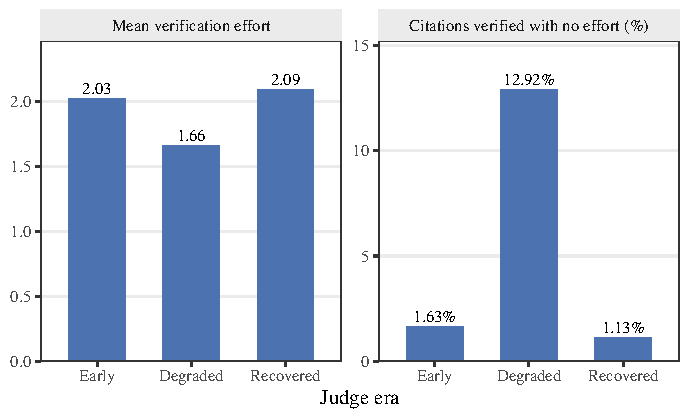
\includegraphics[width=0.57\textwidth]{f3a_era_grounding}\hfill
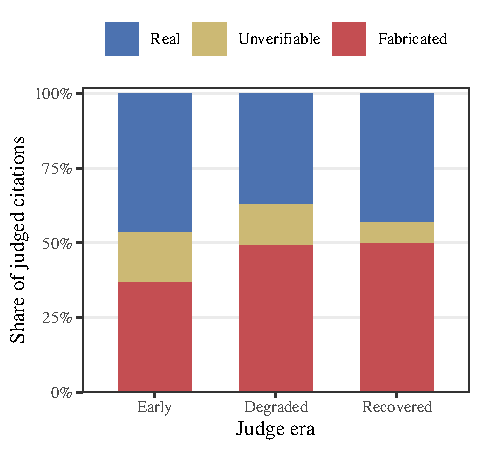
\includegraphics[width=0.40\textwidth]{f3b_era_verdict}
\caption{Judge grounding (left) and verdict mix (right) across the three eras,
over all 31,980 judged citations. The two panels are the point of the figure
read together: grounding falls and then returns to its starting level, while the
verdict distribution steps toward FABRICATED and stays there. An instrument
whose verdicts tracked its grounding would show the right-hand bars returning to
their early-era shape in the third era, and they do not.}
\label{fig:f3}
\end{figure}

\subsection{Does the drift reach the registered contrasts?}
\label{sec:drift-reach}

Balance of era across condition constrains the \emph{mix} of conditions within
each era. It cannot constrain whether the instrument \emph{treats} those
conditions differently, and only the second would bias a registered contrast.
Non-differential misclassification attenuates a contrast toward the null, which
is conservative; differential misclassification can move it either way. So the
question was tested rather than argued. The specification was locked before any
of these models was fitted, era boundaries were fixed from grounding metrics
before this test was specified, and neither is re-tunable to the outcome.

\begin{table}[htbp]
\centering
\small
\caption{Differentiality tests at the complete 31{,}980 judgments. Each takes the
corresponding registered model verbatim and adds the interaction shown; the
statistic is a likelihood-ratio test against that model without it. All four
converged and none is singular.}
\label{tab:t6}
\begin{tabular}{@{}l l r r l l@{}}
\toprule
 & Interaction & $\chi^2$ & df & $p$ & Rejects \\
\midrule
D1 & \texttt{condition} $\times$ era              & 10.074 & 6 & 0.122 & no \\
D2 & \texttt{stage\_ordinal} $\times$ era         & 0.366  & 2 & 0.833 & no \\
D3 & \texttt{condition} $\times$ grounding        & 23.970 & 3 & $2.5 \times 10^{-5}$ & \textbf{yes} \\
D1$'$ & \texttt{condition} $\times$ era, sensitivity \#1 & 10.418 & 6 & 0.108 & no \\
\bottomrule
\end{tabular}
\end{table}

Four things belong in the prose rather than a footnote.

\paragraph{D1 moved, and we report that it moved.}
At an earlier point in judging, on 18{,}364 modeled generations, D1 stood at
$\chi^2 = 13.219$, $p = 0.0397$, and would have rejected. The internal draft
flagged at the time why to distrust it: the terms carrying it were the
recovered-era terms, which had the smallest $n$ and were still accumulating. That
era then grew from 2{,}823 to 5{,}276 generations while the other two did not
change at all, and the test moved to $p = 0.122$, with the interaction now
slightly \emph{worsening} AIC (16084.2 without it against 16086.1 with it). We
state this rather than presenting only the final number. Individual D1 terms
still move around, and they must not be read as significant when the
six-degree-of-freedom omnibus does not reject.

\paragraph{D2 is clean, so E1 is not implicated.}
The stage-by-era interaction is nowhere near rejection ($p = 0.833$). Whatever
the instrument did over time, it did not do it differentially with respect to
post-training stage, which is the axis E1 is estimated on.

\paragraph{D1 and D3 disagree, and the disagreement is informative.}
We do not write that they agree. They now disagree on significance and not merely
on location, and the pre-specification named that possibility in advance as
meaning the answer depends on where the era lines fall. The asymmetry cuts
against reading D3 as the decisive test. Era is a time slice and is exogenous to
the citation; grounding is measured per judgment and is partly a
\emph{consequence} of what was judged, so it is endogenous. The only test that
rejects is the endogenous one. Further, D3's entire signal sits in one condition:
\texttt{abstention\_permitted} at $+0.42$ ($p < 0.0001$), with
\texttt{citations\_expected} at $+0.03$ and \texttt{length\_matched} at $-0.06$,
both indistinguishable from zero. That is the condition in which models cite
least, so the citations surviving there are the most selected, which is exactly
where an endogenous grounding measure would be expected to misbehave.

\paragraph{Sensitivity \#1 attenuates it further.}
Recoding UNVERIFIABLE as fabricated keeps the interaction below detection
($p = 0.108$), with the \texttt{citations\_expected} recovered-era term falling
from $+0.32$ to $+0.10$. That is attenuation, not disappearance, and we word it
that way. It points at the same conclusion the regime table and the paired
sub-study reach independently: the movement runs through the UNVERIFIABLE
channel rather than through a moved REAL-versus-FABRICATED boundary.

\paragraph{What three nulls do not buy.}
These are diagnostics, so we claim no $\alpha$ adjustment across them, and we do
not treat the three non-rejections as a clean bill of health. Power against small
interactions is limited, and a non-significant interaction \emph{bounds} the
evidence for differentiality rather than proving its absence. The tests also
detect differentiality without identifying the direction of any bias, because the
eras contain different items. D3 does reject, so its pre-committed branch
applies: the registered estimands are not adjusted and remain primary, and the
era-stratified robustness panel below re-estimates them under restriction so a
reader can see what the registered contrasts look like inside a single era.

\subsection{The paired re-judge sub-study}

Every analysis above compares different citations judged at different times, so
it cannot separate a change in the instrument from a change in what was being
judged. This sub-study can, because it re-judges the \emph{same} citations.

Five hundred already-judged citations, 250 from each of the first two eras and
balanced across conditions, were re-judged under the recovered instrument with
both verdicts retained. One design detail carries the argument: the re-judge read
the byte-identical prompt file the original judgment used, so
prompt-construction variance is eliminated by construction and any difference in
verdict is attributable to the tool environment rather than to the item or its
rendering.

\begin{table}[htbp]
\centering
\small
\caption{Paired re-judge transition matrices, original verdict to re-judged
verdict, 250 citations per era. The rates are similar across eras; the
composition is not.}
\label{tab:t7}
\begin{tabular}{@{}l rrr c rrr@{}}
\toprule
 & \multicolumn{3}{c}{Early era} & & \multicolumn{3}{c}{Degraded era} \\
\cmidrule(lr){2-4} \cmidrule(lr){6-8}
Original & \multicolumn{3}{c}{re-judged as} & & \multicolumn{3}{c}{re-judged as} \\
 & REAL & FAB. & UNV. & & REAL & FAB. & UNV. \\
\midrule
REAL         & 117 & 3  & 1  & & 102 & 2  & 1 \\
FABRICATED   & 1   & 79 & 3  & & 3   & 101 & 8 \\
UNVERIFIABLE & 2   & 29 & 15 & & 14  & 14 & 5 \\
\bottomrule
\end{tabular}
\end{table}

The differentiality test does not reject in either era: $\chi^2 = 5.077$, df 3,
$p = 0.166$ in the early era and $\chi^2 = 1.376$, df 3, $p = 0.711$ in the
degraded era. Design-reweighted flip rates are close, 0.169 $[0.120, 0.219]$
early and 0.163 $[0.116, 0.211]$ degraded.

Two qualifications are not optional. The test rests on roughly 62 items per
condition cell, so the correct sentence is \textbf{no detectable differentiality
at this power}, never ``proven non-differential.'' And although the flip
\emph{rates} match across eras, their \emph{composition} does not, which
Table~\ref{tab:t7} is included to show. In the early era the traffic is 29
UNVERIFIABLE verdicts becoming FABRICATED against 3 moving the other way; in the
degraded era it is 14 and 14. Direction matters more than volume here, and it is
the same conclusion the sensitivity \#1 attenuation points at: the instrument's
movement runs through the UNVERIFIABLE channel rather than through a shifted
REAL-versus-FABRICATED boundary.

One flag, deliberately not quantified, because it rests on $n = 63$: in the early
era \texttt{citations\_expected} flips at 23.8\% against \texttt{length\_matched}
at 11.3\%. Were that real it would push the amendment \#10 contrast \emph{away}
from the registered-loss bin, which is the opposite direction from the
verifier-REAL trust failure, so the two known biases partially cancel on exactly
that contrast. In the event this is moot: the contrast lands at $+28.4$ points
corrected and $+12.6$ registered, far from any bin boundary, so neither bias nor
their cancellation is load-bearing for the conclusion.

\subsection{Zero-effort robustness}

Some judgments were recorded with zero verification effort, and those skew toward
REAL. The registered robustness check drops them and re-estimates the condition
contrasts. This is \textbf{exploratory}. It is not a substitute for a registered
estimand and we do not present it as one, and like the era-stratified panel it is
gated to run only alongside or after the confirmatory fit.

Dropping those rows takes the modeled set from 20{,}811 generations to
19{,}639, and the picture does not change. Against neutral,
\texttt{citations\_expected} still carries an odds ratio of \textbf{8.18}
$[7.14, 9.37]$, while \texttt{length\_matched} sits at \textbf{1.18}
$[1.05, 1.32]$. The ordering that matters for the de-confounding argument, the
citation cue far above the length demand, survives the check intact.

\paragraph{Most of the era-stratified panel is not estimable, and we say so
rather than reading it as null.} Re-fitting the registered condition model inside
a single era leaves several contrasts degenerate. In the degraded era
\texttt{citations\_expected} versus neutral returns an odds ratio of 9.1 with a
95\% interval running from below $10^{-3}$ to above $10^{9}$; in the recovered
era it returns 13.5 with a comparably useless interval; and
\texttt{abstention\_permitted} is inestimable in every stratum, including the
pooled zero-effort fit, where its interval spans ten orders of magnitude. An
estimate like that carries a large $p$-value, and \textbf{a large $p$-value here
means the model could not identify the coefficient, not that the effect is
absent}. Reading those cells as evidence of a vanishing citation effect would be
exactly backwards.

Only two things in the panel are interpretable. \texttt{length\_matched} versus
neutral is estimable in all three eras (1.02 $[0.87, 1.20]$ early, 1.43
$[1.11, 1.83]$ degraded, 1.40 $[1.11, 1.76]$ recovered), and
\texttt{citations\_expected} versus neutral is estimable in the early era at 8.59
$[7.15, 10.31]$. That is a thin result and we report it as one.

We flag a limitation of the diagnostic itself, because it affects how these rows
should be read. The panel marks a contrast as separated when its standard error
exceeds 100, which is far too permissive: a standard error near 6 already yields
an odds-ratio interval spanning ten orders of magnitude while passing that test
unflagged. The separation flags in the artifact therefore understate how many
cells are degenerate, and the judgment above rests on interval width rather than
on the flag.
